\documentclass[11pt,a4paper]{article}
\usepackage[margin=23mm,headheight=15pt]{geometry}
\usepackage[T1]{fontenc}
\usepackage{lmodern,microtype,booktabs,tabularx,longtable,graphicx,xcolor,hyperref,fancyhdr,enumitem,caption,titlesec,tcolorbox}
\tcbuselibrary{breakable,skins}
\definecolor{ink}{HTML}{172B4D}
\definecolor{teal}{HTML}{137C8B}
\definecolor{coral}{HTML}{E76F51}
\definecolor{mist}{HTML}{F1F6F8}
\hypersetup{colorlinks=true,linkcolor=teal,urlcolor=teal,citecolor=teal}
\setlength{\parindent}{0pt}\setlength{\parskip}{7pt}\setlength{\emergencystretch}{3em}
\pagestyle{fancy}\fancyhf{}\lhead{\textcolor{teal}{IDM-Viz}}\rhead{Phase 3 -- Research supplement}\cfoot{\thepage}
\titleformat{\section}{\Large\bfseries\color{ink}}{\thesection}{.6em}{}
\titleformat{\subsection}{\large\bfseries\color{teal}}{\thesubsection}{.6em}{}
\captionsetup{font=small,labelfont={bf,color=ink}}
\newcommand{\EstimatorResults}{
\begin{tabular}{lrrr}
\toprule
Estimator & MAE [95\% seed CI] & Bias & Cal. interval coverage \\ \midrule
CAL & 0.0913 [0.0901, 0.0924] & +0.0381 & 0.632 \\
RAW & 0.0908 [0.0895, 0.0921] & +0.0409 & 0.632 \\
ATC & 0.1201 [0.1162, 0.1238] & +0.0469 & 0.632 \\
CONSTANT & 0.0931 [0.0922, 0.0941] & +0.0299 & 0.632 \\
\bottomrule
\end{tabular}
}
\newcommand{\DetectorResults}{
\begin{tabular}{llrrr}
\toprule
Regime & Detector & False alarm rate & Detection rate & Mean lag (batches) \\ \midrule
M0 stationary & KS/PCA & 0.048 & 0.978 & 22.25 \\
M0 stationary & Pairwise correlation & 0.066 & 0.889 & 15.75 \\
M1 abrupt nuisance & KS/PCA & 0.048 & 1.000 & 0.00 \\
M1 abrupt nuisance & Pairwise correlation & 0.066 & 0.889 & 15.75 \\
M2 gradual predictive & KS/PCA & 0.048 & 1.000 & 2.27 \\
M2 gradual predictive & Pairwise correlation & 0.066 & 0.889 & 15.75 \\
M3 incremental repeated small & KS/PCA & 0.048 & 1.000 & 0.11 \\
M3 incremental repeated small & Pairwise correlation & 0.066 & 0.889 & 15.75 \\
M4 abrupt conditional reversal & KS/PCA & 0.048 & 0.978 & 22.25 \\
M4 abrupt conditional reversal & Pairwise correlation & 0.066 & 0.889 & 15.75 \\
M5 recurrent conditional reversal & KS/PCA & 0.048 & 0.978 & 22.25 \\
M5 recurrent conditional reversal & Pairwise correlation & 0.066 & 0.889 & 15.75 \\
M6 dependence marginals preserved & KS/PCA & 0.048 & 0.978 & 11.40 \\
M6 dependence marginals preserved & Pairwise correlation & 0.066 & 1.000 & 0.03 \\
M7 out of support & KS/PCA & 0.048 & 1.000 & 0.00 \\
M7 out of support & Pairwise correlation & 0.066 & 0.889 & 15.75 \\
\bottomrule
\end{tabular}
}
\newcommand{\DelayResults}{
\begin{tabular}{rrrrr}
\toprule
Delay & Age at release & Accuracy after release & Verified harm fraction & Verified batches \\ \midrule
0 & 0 & 0.578 & 0.233 & 11,520 \\
5 & 5 & 0.578 & 0.233 & 11,520 \\
20 & 20 & 0.578 & 0.233 & 11,520 \\
100 & 100 & 0.578 & 0.233 & 11,520 \\
\bottomrule
\end{tabular}
}
\newcommand{\ReleasedErrorResults}{
\begin{tabular}{rrrrr}
\toprule
Delay & Stationary false alarm & Drift detected by input end & Drift detected after drain & Mean lag (source batches) \\ \midrule
0 & 0.000 & 0.487 & 0.487 & 5.66 \\
5 & 0.000 & 0.487 & 0.487 & 5.66 \\
20 & 0.000 & 0.487 & 0.487 & 5.66 \\
100 & 0.000 & 0.000 & 0.487 & 5.66 \\
\bottomrule
\end{tabular}
}
\newcommand{\PairedResults}{
\begin{tabular}{lrrr}
\toprule
Comparator & Mean paired $\Delta$MAE & Holm $q<.05$ strata & Strata \\ \midrule
CAL $-$ RAW & +0.0001 & 37 & 120 \\
CAL $-$ ATC & -0.0257 & 99 & 120 \\
CAL $-$ CONSTANT & -0.0019 & 12 & 120 \\
\bottomrule
\end{tabular}
}
\newcommand{\DimensionSensitivity}{}

\begin{document}
\begin{titlepage}\color{ink}
\vspace*{12mm}{\large\textcolor{teal}{DATA ANALYSIS AND VISUALIZATION -- PHASE 3}}\\[18mm]
{\Huge\bfseries IDM-Viz}\\[4mm]
{\LARGE Impact-aware drift monitoring under delayed feedback}\\[8mm]
{\Large A controlled robustness and evidence-quality evaluation}\\[20mm]
\begin{tcolorbox}[colback=mist,colframe=teal,boxrule=0pt,leftrule=2.2mm,arc=1.5mm]
\textbf{Study design}\\
3 synthetic task families; 8 paired mechanisms; 30 held-out seeds; 500-row batches; 96 input batches; four label-delay schedules.
\end{tcolorbox}
\vfill
\textbf{Ahmed Bilal (23I-2581) -- Umar Behram (23I-2604)}\\
FAST-NUCES Islamabad\\[4mm]
Supplementary report -- 16 November 2026\\
Editable source: \texttt{REPORT.tex}
\end{titlepage}
\tableofcontents\clearpage
\begin{abstract}
This supplementary evaluation strengthens the Phase 3 implementation with paired, controlled drift mechanisms and an explicit input-before-label release runner. It compares a frozen isotonic Average-Confidence estimator with raw confidence, an ATC-style estimator and historical accuracy; measures original-feature/PCA and pairwise-correlation input evidence; and verifies cached predictions after delays of 0, 5, 20 and 100 batches. The locked held-out matrix contains \textbf{720 complete task--mechanism--seed cells}; the primary comparison uses eight features and \textbf{30 independent seed blocks}. Results are conditional on the stated synthetic laws. They do not establish general transfer, causal attribution, certified harm probability, future-risk performance, or improved analyst decisions.
\end{abstract}

\begin{tcolorbox}[breakable,colback=mist,colframe=ink,boxrule=.4pt,title=Interpretation at a glance]
All reported numbers are generated from checksummed cell artifacts. Point estimates and 95\% intervals resample complete seeds, never batches or delay copies. The estimator aggregates over the two predeclared post-intervention phases. The exact evidence, locked source snapshot and run state are available in the accompanying result directory. The coordinated view is described as a prototype; no analyst-benefit claim is made.
\end{tcolorbox}

\section{Phase 2 basis and changes}
The team's submitted Phase 2 DOCX remains the authoritative methodological basis and is byte-for-byte preserved (SHA-256: \texttt{786d4f23\allowbreak{}d54d0d09\allowbreak{}edd5f947\allowbreak{}40198f43\allowbreak{}ca3b406e\allowbreak{}b38626ae\allowbreak{}754fe04f\allowbreak{}e26c5ef4}). No instructor feedback was received. This supplement adds controlled tests to the integrated IDM-Viz objective; it does not replace the submitted research question or earlier reports.

The implementation uses a frozen logistic classifier; historical-only scaler, PCA, clustering and correctness calibration; 4,000 training, 2,000 calibration and 2,000 fixed-reference observations; and paired generators. PCA replaces the proposed autoencoder. Original-feature and correlation statistics are descriptive, not causal. Weather was not admitted because its primary source, ordering, label construction and checksum remain unverified. Causal discovery, broad adaptation and deployment validation are outside this run. The coordinated view is reported as a prototype, with no claim of improved analyst performance.

\section{Experimental setup}
The primary held-out design crosses the linear probabilistic, XOR nonlinear, and five-region generating families with: stationary control; abrupt nuisance-feature shift; gradual predictive-feature shift; repeated small shifts; abrupt conditional reversal; recurrent conditional reversal; dependence change with preserved marginal scales; and a large covariate displacement. Each stream has 96 batches of 500 rows. Batches 1--24 are a shared stationary prefix across mechanisms within a task/seed. Interventions begin at batch 25; the gradual change reaches its specified endpoint at batch 40; the recurrent conditional reversal returns during batches 65--80. The five-region ID and the true label probability are evaluator-only. The locked M7 identifier says ``out of support'', but the Gaussian source has unbounded support: M7 is interpreted only as a finite-sample low-density extrapolation stress, not a literal support violation.

Seeds are paired across mechanisms and disjoint from development/validation banks. A frozen logistic model is fitted once on historical training rows; the isotonic correctness map uses only its separate calibration rows. KS/PCA and correlation detectors receive only current features. The correlation threshold is calibrated from pseudo-cohorts in the historical calibration partition against the fixed reference features. The probability interval is an exact plug-in Poisson-binomial distribution that treats correctness probabilities as fixed. It is not a confidence interval accounting for calibration or reference uncertainty. A small-window, released-error ADWIN-style detector is also scored when labels arrive; it uses a transparent exact split scan and is not the compressed River ADWIN implementation.

At each input clock, scores and predictions are computed and persisted before any labels scheduled for that clock are released. The release replay validates prediction/label row identifiers and drains the queue after the final input batch without fabricating new input. Delay changes when verification is available; this frozen-model comparison does not allow delayed labels to change earlier predictions.

\section{Accuracy-estimation results}
Table~\ref{tab:estimators} averages each estimator's batch-level absolute error and bias over batches 25--40 and 65--80, then averages matched conditions within each seed. The interval is a 2,000-replicate percentile bootstrap over seed blocks. Coverage is the empirical fraction of batch accuracies inside the plug-in interval; width is descriptive.
\begin{table}[htbp]\centering\small\EstimatorResults\caption{Held-out accuracy estimation, eight-feature primary setting.}\label{tab:estimators}\end{table}

The comparison is internal and paired. Raw Average Confidence and ATC-style thresholding are within-study comparators, not fresh replications of published benchmarks. The calibrated correctness-probability Brier score is 0.2483 [0.2478, 0.2488] (95\% seed-bootstrap interval). The calibration map is learned under a historical source law and can fail when the conditional relationship between confidence and correctness changes. High confidence must not be presented as verified accuracy. The interval-coverage column evaluates the calibrated plug-in interval and is therefore repeated for point-estimator comparators.

Table~\ref{tab:paired} summarizes paired seed-level sign-flip tests. The family-wide Holm correction covers the complete predeclared primary set of task, mechanism, phase, and comparator contrasts. Negative mean differences favor the calibrated estimator; significance counts are descriptive across strata, not independent replications. Across the primary strata, mean paired calibrated-minus-raw MAE was +0.0001; against ATC-style it was -0.0257; against the historical constant it was -0.0019. This means the isotonic estimator did not uniformly dominate the baselines, so the evidence supports a comparative trade-off rather than a universal calibration advantage.
\begin{table}[htbp]\centering\small\PairedResults\caption{Paired primary-setting estimator contrasts; $\Delta$MAE is calibrated minus comparator.}\label{tab:paired}\end{table}

\DimensionSensitivity
\section{Input detection and descriptive localization}
Table~\ref{tab:detection} reports seed-averaged false-alarm rates over the stationary prefix and any-alarm detection after the programmed intervention. Detection delay is measured from batch 25, so it is not a valid onset-latency summary for mechanisms whose effect is gradual, recurrent, or conditionally localized. The correlation detector is a project-specific maximum absolute pairwise correlation-change statistic, not ADWIN or a reproduction of a named detector.
\begin{table}[htbp]\centering\scriptsize\resizebox{\linewidth}{!}{\DetectorResults}\caption{Input-evidence trade-offs by programmed mechanism.}\label{tab:detection}\end{table}

\begin{figure}[p]\centering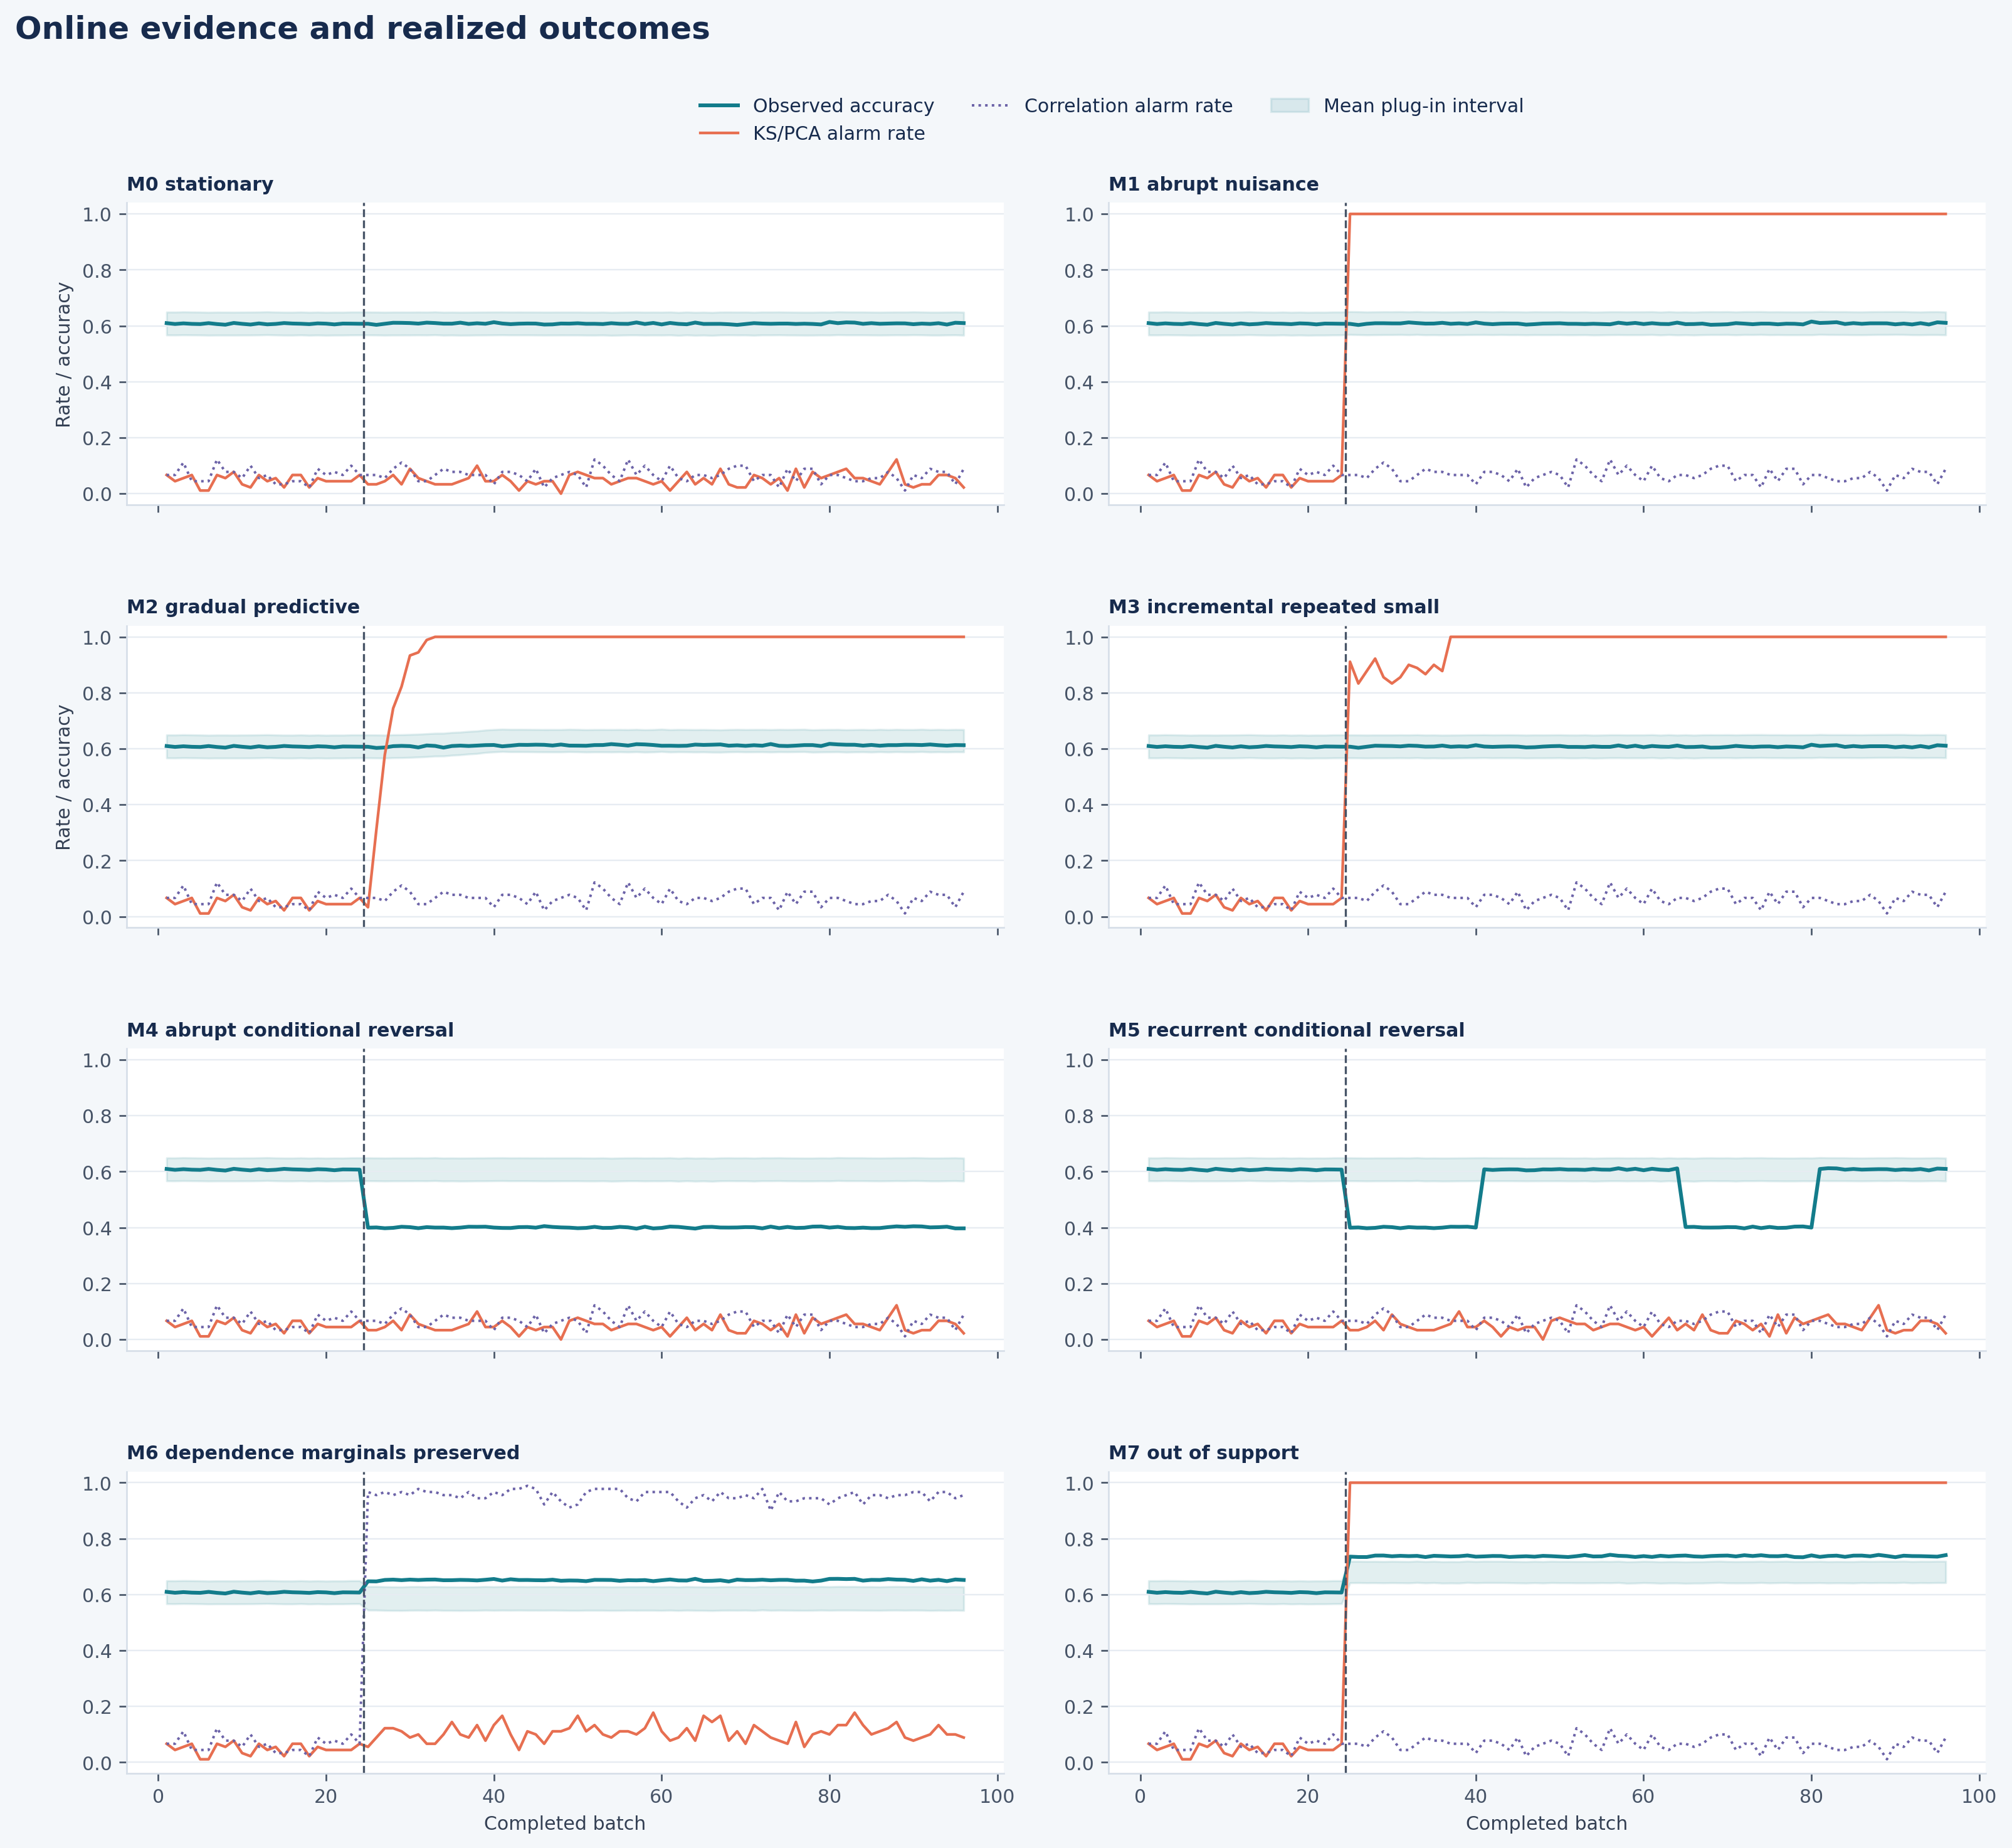
\includegraphics[width=\linewidth,height=.86\textheight,keepaspectratio]{figures/fig02_detection_and_accuracy_timeline.png}\caption{Batch-level accuracy, input alarms and plug-in interval across all mechanisms. The vertical marker indicates the end of the shared stationary prefix. Alarm rates and outcome truth are aggregated across tasks and seeds.}\end{figure}

Feature ranks are descriptive. Precision@1 and recall@3 are defined only where the generator specifies changed marginal features. They are undefined for pure dependence and conditional-only changes. The five-region task keeps region truth out of the online scorer; no cluster-to-region accuracy is claimed.
\begin{figure}[htbp]\centering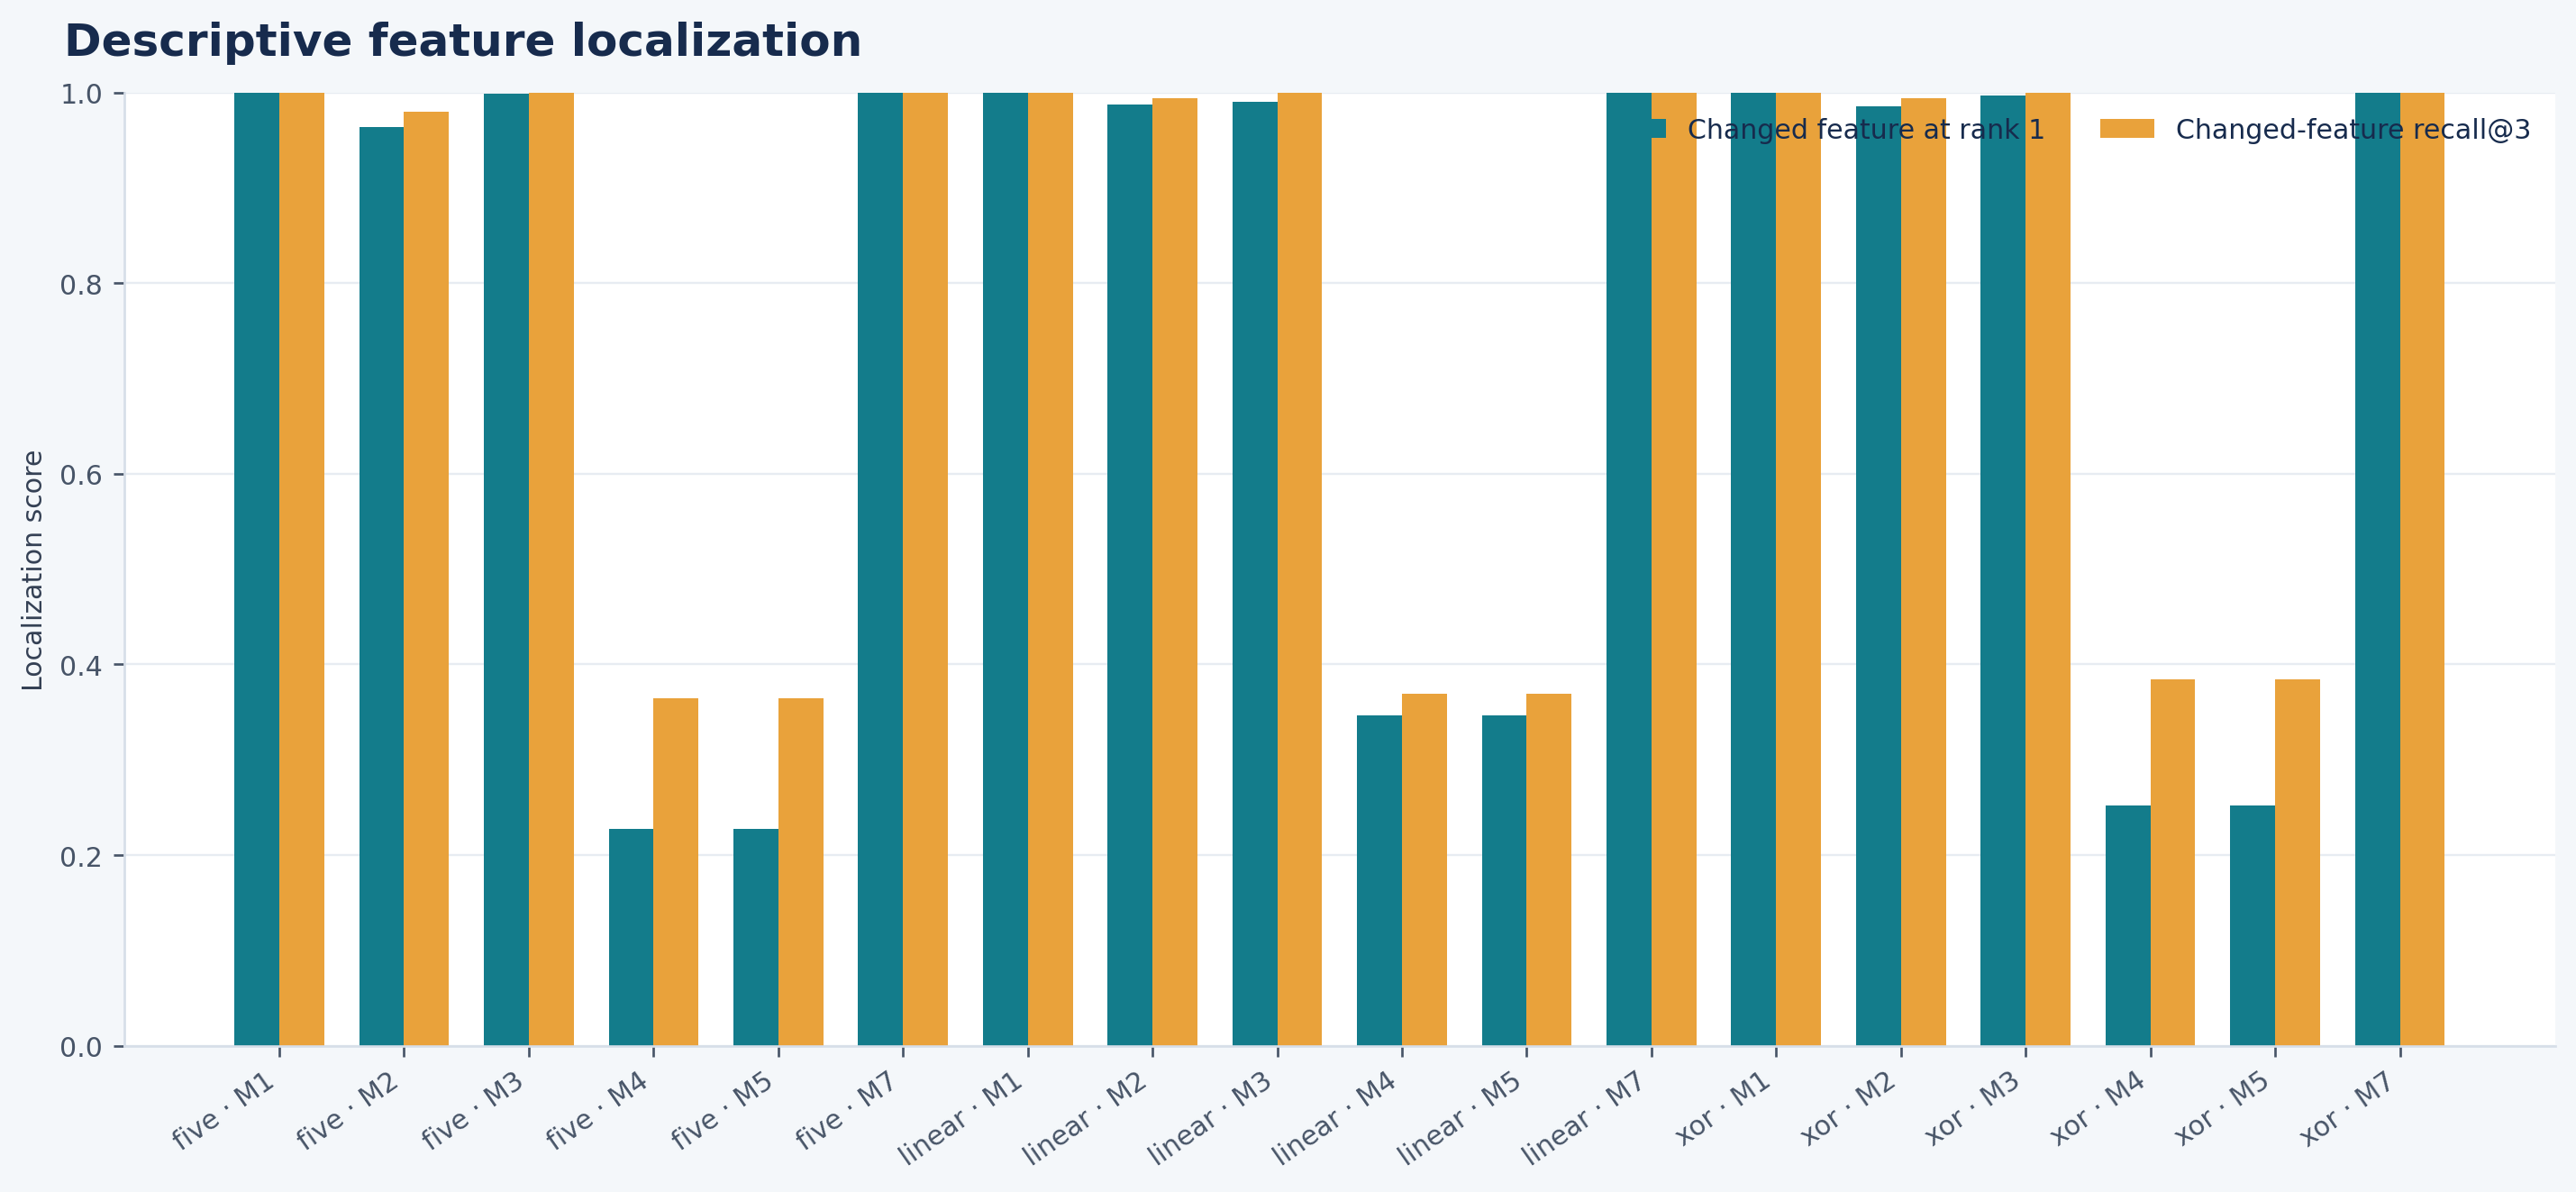
\includegraphics[width=.96\linewidth]{figures/fig04_feature_localization.png}\caption{Changed-feature retrieval in mechanisms with known marginal targets. This is not causal attribution.}\end{figure}

\section{Delayed-label verification}
Table~\ref{tab:delay} shows released evidence age and verified outcomes for the early post-intervention phase. All 96 cohorts in every cell are eventually verified after queue drainage. Delay 100 therefore means no labels arrive during the 96-batch input period; results after drainage are retrospective verification, not online evidence.
\begin{table}[htbp]\centering\small\DelayResults\caption{Verification at the scheduled release clock.}\label{tab:delay}\end{table}
The released-error comparator sees a verified cohort only after its scheduled availability time. For each release it scans eligible historical window cuts with a Hoeffding difference bound, trims the older segment after an alarm, and retains the newer segment. Table~\ref{tab:released-error} separates detection before the 96-batch input horizon from detection after the 100-batch queue drains. This is an explicitly project-defined ADWIN-style comparator, not a reproduction of River ADWIN.
\begin{table}[htbp]\centering\small\resizebox{\linewidth}{!}{\ReleasedErrorResults}\caption{Released-error detector outcomes by scheduled delay.}\label{tab:released-error}\end{table}
\begin{figure}[htbp]\centering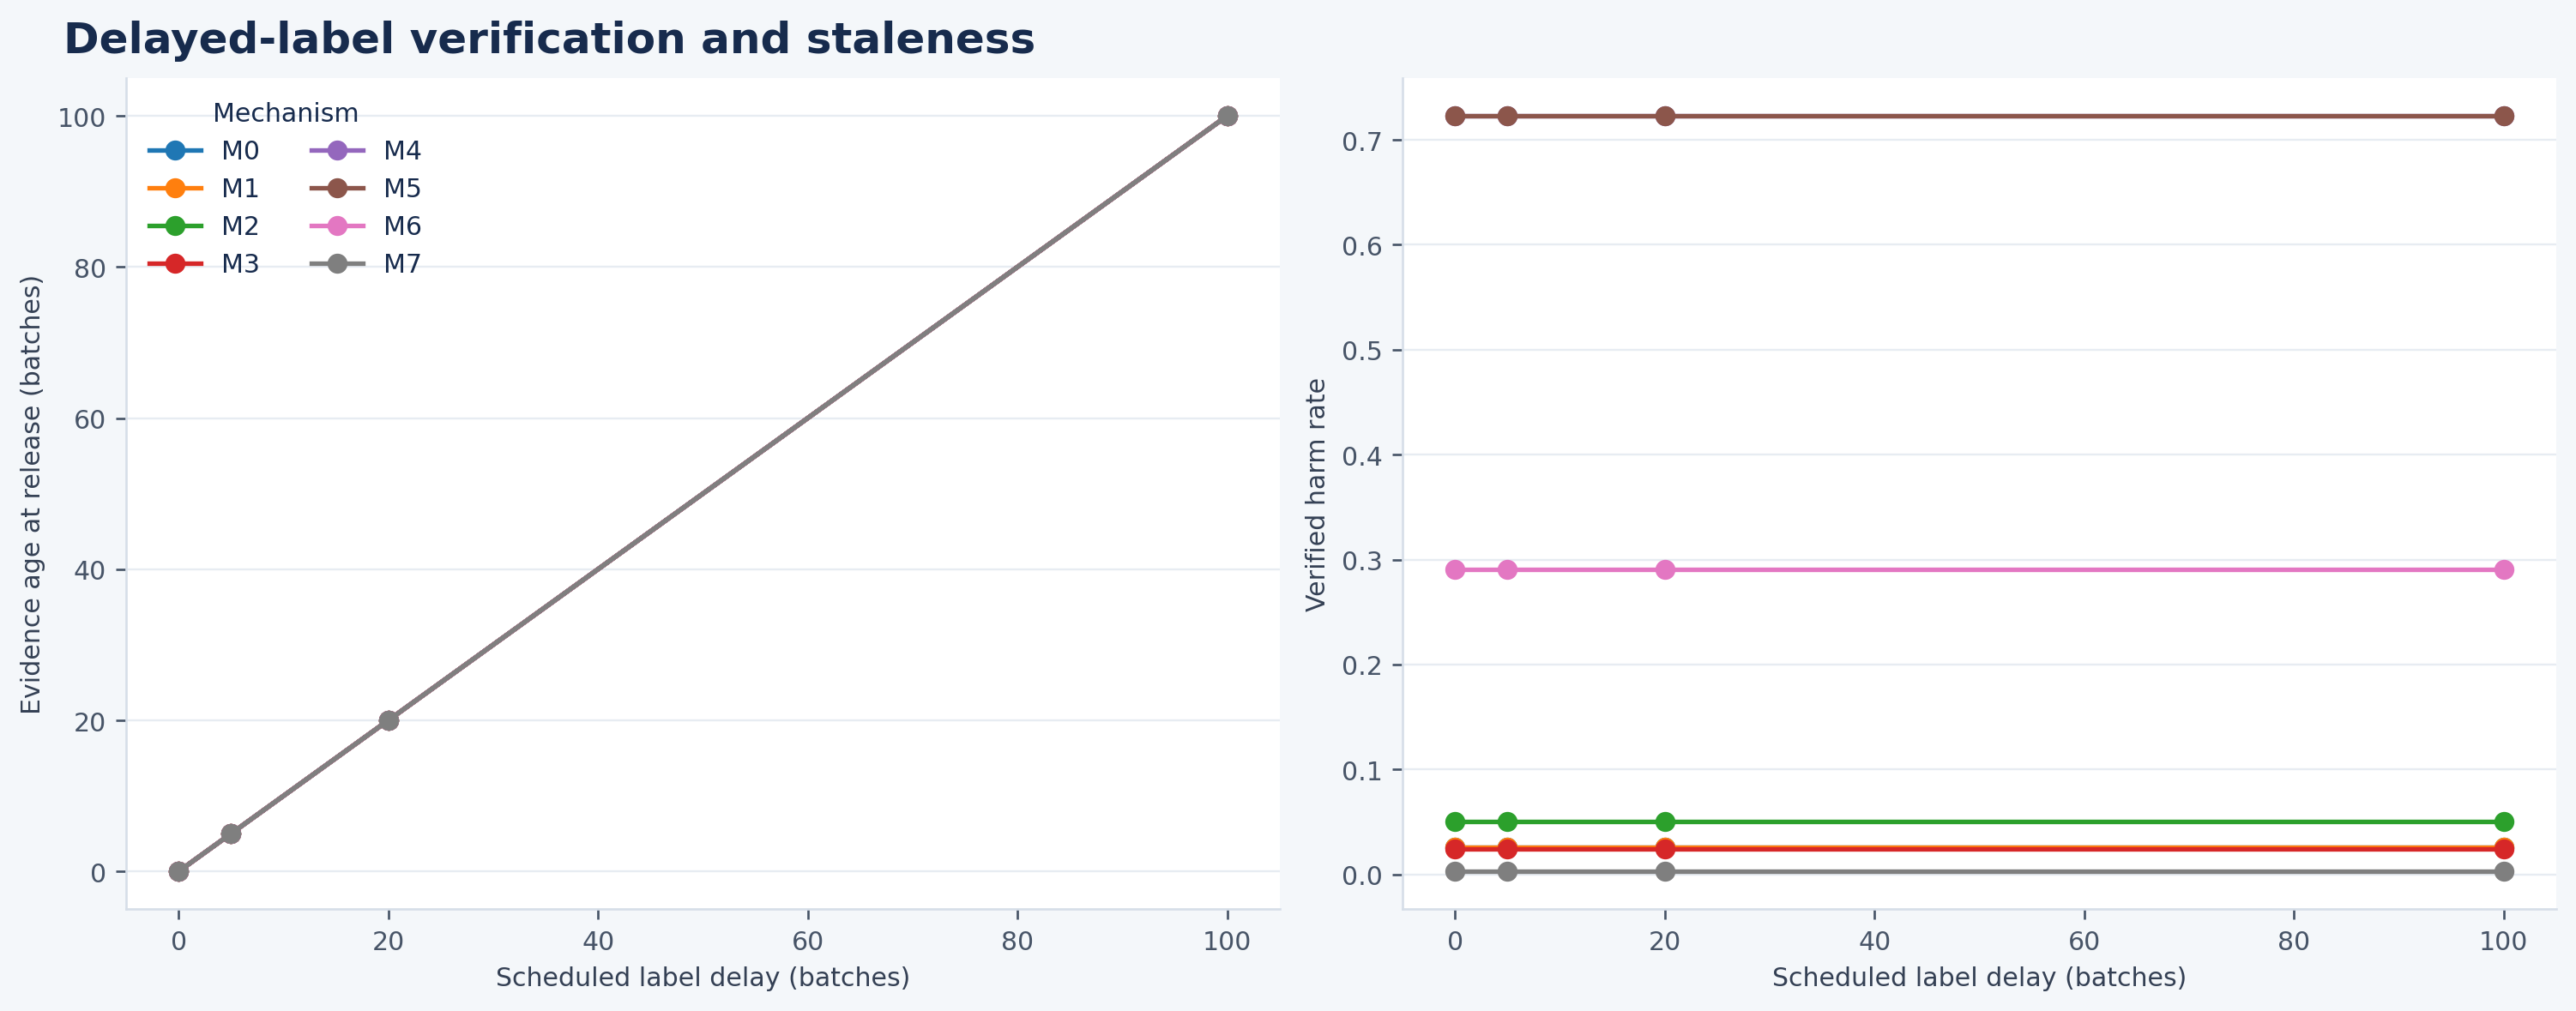
\includegraphics[width=.96\linewidth]{figures/fig03_delay_verification.png}\caption{Release age and retrospective verified harm across the four delay settings.}\end{figure}

\section{Statistical analysis and reproducibility}
Complete seeds are the resampling unit. Point estimates use equal weight per seed after averaging the predeclared stream cells; a batch is not an independent replicate. Estimator contrasts are paired within seeds and Holm adjusted across the declared contrast family. Detector operating rates are reported by mechanism to avoid conflating high sensitivity with general quality. A full analysis manifest provides source hashes, exact cell count, bootstrap configuration, CSV checksums and figure checksums.

Reproduce from the project root with the Anaconda environment used for the measured run:
\begin{verbatim}
python scripts/run_strengthening_v3.py --profile evaluation \\
  --output results/phase3/reproduction_evaluation_d8
python scripts/analyze_strengthening_v3.py \\
  results/phase3/reproduction_evaluation_d8
python scripts/build_strengthening_report.py \\
  results/phase3/reproduction_evaluation_d8 \\
  --output reports/phase3/reproduction_evaluation_d8
\end{verbatim}
Do not reuse an existing output directory for a new run. Resume only an interrupted run with the same lock, source snapshots and expected cells by adding \texttt{--resume}.

\section{Comparison with research and limits}
The classical accuracy-estimation literature emphasizes that unlabeled target performance requires assumptions about the source/target relationship; see Garg et al. (2022). Work on uncertainty under dataset shift similarly cautions that source calibration does not guarantee target reliability (Ovadia et al., 2019). This experiment contributes a controlled, label-safe comparison within its own generator laws; it does not transfer numerical rankings from those studies because their datasets, models, splits and estimands differ.

The five-region and conditional mechanisms test heterogeneous and label-law changes synthetically, not natural environments. The concern score uses plug-in probabilities and a selected harm margin; it is not calibrated risk or a population guarantee. The correlation alarm may increase stationary alert burden. No result here identifies causality, proves transfer to the pending weather stream, validates all named literature baselines, or measures decision quality. The prior v5 consolidated report and external-data supplements remain separate and unchanged; this report adds a versioned extension rather than replacing their results.

\begin{thebibliography}{9}
\bibitem{garg2022}S. Garg et al., ``Leveraging Unlabeled Data to Predict Out-of-Distribution Performance,'' 2022. \url{https://arxiv.org/abs/2201.04234}
\bibitem{ovadia2019}Y. Ovadia et al., ``Can You Trust Your Model's Uncertainty? Evaluating Predictive Uncertainty Under Dataset Shift,'' NeurIPS, 2019. \url{https://proceedings.neurips.cc/paper/2019/hash/8558cb408c1d76621371888657d2eb1d-Abstract.html}
\end{thebibliography}
\end{document}
